The Standard Model is the most comprehensive theory of particle physics that describes the fundamental particles and their interactions. It is a quantum field theory that unifies all fundamental particles and their interactions into a single, cohesive framework --- excluding only gravity. The Standard Model emerged not from a single discovery or individual, but through the collective efforts of countless experimental and theoretical physicists over several decades of the 20th century.

The Standard Model accurately describes three of the four fundamental forces of nature: electromagnetism, the weak nuclear force, and the strong nuclear force, as particle interactions. The fourth force, gravity, remains outside the Standard Model despite many attempts to develop a quantum formalism for it. Instead, gravity is described by Einstein's theory of general relativity~\cite{GR_review_article} where it manifests itself as the curvature of spacetime. Within the Standard Model, the fundamental particles are categorized into two groups: bosons, and fermions.

A boson is a subatomic particle with an integer spin quantum number that obeys Bose-Einstein statistics. A vector boson is a special case of a boson and consists of spin-1 particles. There are four types of such vector bosons in the SM:\@ the photon ($\gamma$), the $W^{\pm}$ and $Z$ bosons, and the gluon ($g$). The photon is massless and mediates the electromagnetic force (Section~\ref{sec:theory_qed}). The $W^{\pm}$ and $Z$ bosons are massive particles that mediate the weak nuclear force. The $W^\pm$ bosons are electrically charged where the $Z$ boson is neutral, and slightly more massive (Section~\ref{sec:theory_ew}). The gluon is massless and mediates the strong nuclear force (Section~\ref{sec:theory_qcd}). Additionally, there are scalar bosons, which are bosons with spin-0. The only known scalar boson in the Standard Model is the Higgs boson ($H$) (Section~\ref{sec:theory_higgs_mechanism}).

A fermion is a subatomic particle with a half-integer spin quantum number that follow Fermi-Dirac statistics. In the Standard Model, fermions are divided into two categories: quarks and leptons. Each category is further split into three generations, with each generation containing a pair of quarks and a pair of leptons. Particles in higher generations are more massive than the previous generation, but share the same quantum numbers and interactions. There are 12 fermions in total, 6 quarks and 6 leptons. The leptons are divided into charged lepton---neutrino pairs, where each lepton is associated with a corresponding neutrino. The charged leptons are the electron ($e^{-}$), muon ($\mu^{-}$), and tau ($\tau^{-}$), with respective neutrinos being electron neutrino ($\nu_{e}$), muon neutrino ($\nu_{\mu}$), and tau neutrino ($\nu_{\tau}$). Additionally, each lepton has a corresponding antiparticle, $e^{+}$, $\mu^{+}$, $\tau^{+}$, $\bar{\nu}_{e}$, $\bar{\nu}_{\mu}$, and $\bar{\nu}_{\tau}$. 
The quarks are similarly divided into ``up'' and ``down'' type quarks. The up-type quarks are the up ($u$), charm ($c$), and top ($t$) quarks, while the down-type quarks are the down ($d$), strange ($s$), and bottom ($b$) quarks. Each quark has a corresponding antiparticle: $\bar{u}$, $\bar{c}$, $\bar{t}$, $\bar{d}$, $\bar{s}$, and $\bar{b}$. Like leptons, quarks are electrically charged ($\frac{2}{3}$ for ``up'' types, $-\frac{1}{3}$ for ``down'' types) but they also carry color charge due to their interactions with the strong nuclear force.

The Standard Model is summarized in Figure~\ref{fig:standard_model}. To understand the structure and symmetries of the Standard Model, it is necessary to first introduce the mathematical foundations, which are presented in Section~\ref{sec:theory_groups}. After this, an overview of the essential components of the Standard Model is provided in Sections~\ref{sec:theory_qed},~\ref{sec:theory_qcd}, and~\ref{sec:theory_ew}. The chapter concludes with a discussion of the Higgs boson, including its production mechanisms and decay channels.

\begin{figure}[htp]
    \centering
    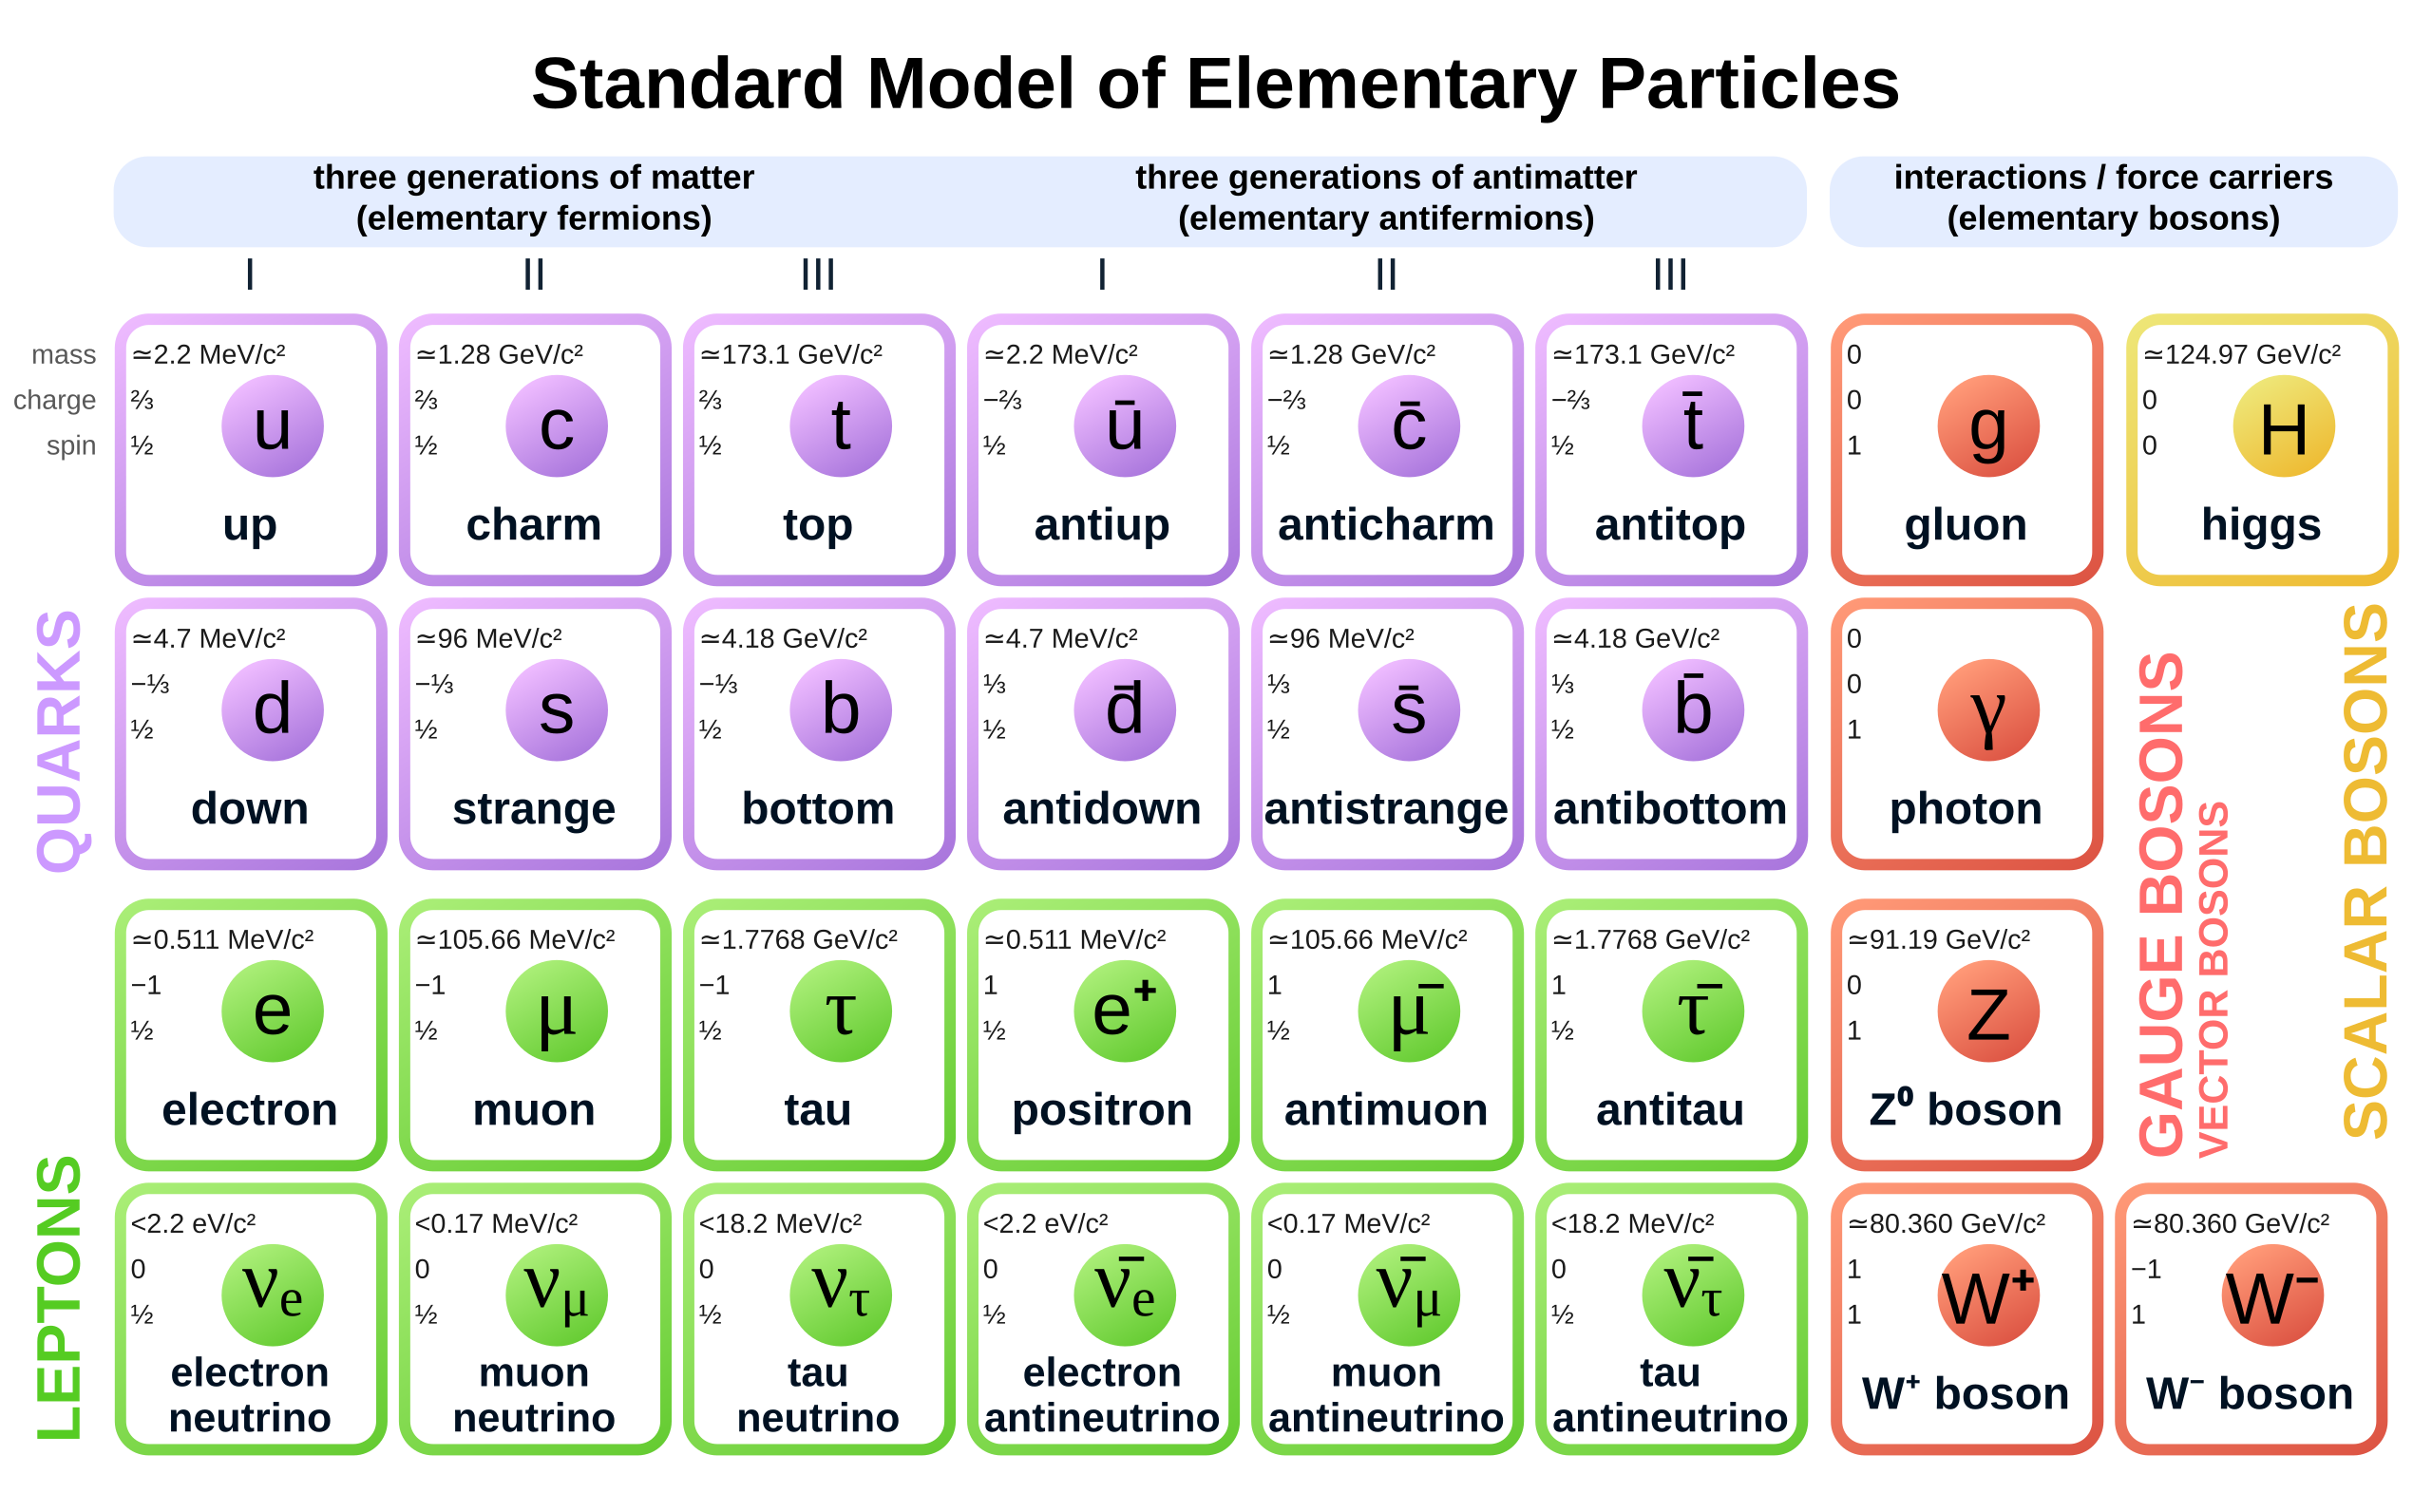
\includegraphics[width=0.8\textwidth]{figures/theory/theory_standard_model.png}
    \caption{Depicted is the visual version of the Standard Model. The elementary particles are grouped via fermions and bosons. Fermions are further divided into quarks and leptons. The bosons are divided into gauge bosons and the Higgs boson. Additionally, the corresponding antiparticles are shown. Taken from~\cite{theory_sm_figure}.}\label{fig:standard_model}
\end{figure}